\documentclass{ximera}

%\usepackage{todonotes}

\newcommand{\todo}{}

\usepackage{tkz-euclide}
\tikzset{>=stealth} %% cool arrow head
\tikzset{shorten <>/.style={ shorten >=#1, shorten <=#1 } } %% allows shorter vectors

\usepackage{tkz-tab}  %% sign charts
\usetikzlibrary{decorations.pathreplacing} 

\usetikzlibrary{backgrounds} %% for boxes around graphs
\usetikzlibrary{shapes,positioning}  %% Clouds and stars
\usetikzlibrary{matrix} %% for matrix
\usepgfplotslibrary{polar} %% for polar plots
\usetkzobj{all}
\usepackage[makeroom]{cancel} %% for strike outs
%\usepackage{mathtools} %% for pretty underbrace % Breaks Ximera
\usepackage{multicol}

\usepackage{polynom}



\usepackage[many]{tcolorbox}  %% for titled boxes
\newtcolorbox{xbox}[1]{%
    tikznode boxed title,
    enhanced,
    arc=0mm,
    interior style={white},
    attach boxed title to top center= {yshift=-\tcboxedtitleheight/2},
    fonttitle=\bfseries,
    colbacktitle=white,coltitle=black,
    boxed title style={size=normal,colframe=white,boxrule=0pt},
    title={#1}}


\usepackage{array}
\setlength{\extrarowheight}{+.1cm}   
\newdimen\digitwidth
\settowidth\digitwidth{9}
\def\divrule#1#2{
\noalign{\moveright#1\digitwidth
\vbox{\hrule width#2\digitwidth}}}





\newcommand{\RR}{\mathbb R}
\newcommand{\R}{\mathbb R}
\newcommand{\N}{\mathbb N}
\newcommand{\Z}{\mathbb Z}

%\renewcommand{\d}{\,d\!}
\renewcommand{\d}{\mathop{}\!d}
\newcommand{\dd}[2][]{\frac{\d #1}{\d #2}}
\newcommand{\pp}[2][]{\frac{\partial #1}{\partial #2}}
\renewcommand{\l}{\ell}
\newcommand{\ddx}{\frac{d}{\d x}}
\newcommand{\ddt}{\frac{d}{\d t}}

\newcommand{\zeroOverZero}{\ensuremath{\boldsymbol{\tfrac{0}{0}}}}
\newcommand{\inftyOverInfty}{\ensuremath{\boldsymbol{\tfrac{\infty}{\infty}}}}
\newcommand{\zeroOverInfty}{\ensuremath{\boldsymbol{\tfrac{0}{\infty}}}}
\newcommand{\zeroTimesInfty}{\ensuremath{\small\boldsymbol{0\cdot \infty}}}
\newcommand{\inftyMinusInfty}{\ensuremath{\small\boldsymbol{\infty - \infty}}}
\newcommand{\oneToInfty}{\ensuremath{\boldsymbol{1^\infty}}}
\newcommand{\zeroToZero}{\ensuremath{\boldsymbol{0^0}}}
\newcommand{\inftyToZero}{\ensuremath{\boldsymbol{\infty^0}}}



\newcommand{\numOverZero}{\ensuremath{\boldsymbol{\tfrac{\#}{0}}}}
\newcommand{\dfn}{\textbf}
%\newcommand{\unit}{\,\mathrm}
\newcommand{\unit}{\mathop{}\!\mathrm}
\newcommand{\eval}[1]{\bigg[ #1 \bigg]}
\newcommand{\seq}[1]{\left( #1 \right)}
\renewcommand{\epsilon}{\varepsilon}
\renewcommand{\iff}{\Leftrightarrow}

\DeclareMathOperator{\arccot}{arccot}
\DeclareMathOperator{\arcsec}{arcsec}
\DeclareMathOperator{\arccsc}{arccsc}
\DeclareMathOperator{\si}{Si}
\DeclareMathOperator{\proj}{proj}
\DeclareMathOperator{\scal}{scal}


\newcommand{\tightoverset}[2]{% for arrow vec
  \mathop{#2}\limits^{\vbox to -.5ex{\kern-0.75ex\hbox{$#1$}\vss}}}
\newcommand{\arrowvec}[1]{\tightoverset{\scriptstyle\rightharpoonup}{#1}}
\renewcommand{\vec}{\mathbf}
\newcommand{\veci}{\vec{i}}
\newcommand{\vecj}{\vec{j}}
\newcommand{\veck}{\vec{k}}
\newcommand{\vecl}{\boldsymbol{\l}}

\newcommand{\dotp}{\bullet}
\newcommand{\cross}{\boldsymbol\times}
\newcommand{\grad}{\boldsymbol\nabla}
\newcommand{\divergence}{\grad\dotp}
\newcommand{\curl}{\grad\cross}
%\DeclareMathOperator{\divergence}{divergence}
%\DeclareMathOperator{\curl}[1]{\grad\cross #1}


\colorlet{textColor}{black} 
\colorlet{background}{white}
\colorlet{penColor}{blue!50!black} % Color of a curve in a plot
\colorlet{penColor2}{red!50!black}% Color of a curve in a plot
\colorlet{penColor3}{red!50!blue} % Color of a curve in a plot
\colorlet{penColor4}{green!50!black} % Color of a curve in a plot
\colorlet{penColor5}{orange!80!black} % Color of a curve in a plot
\colorlet{fill1}{penColor!20} % Color of fill in a plot
\colorlet{fill2}{penColor2!20} % Color of fill in a plot
\colorlet{fillp}{fill1} % Color of positive area
\colorlet{filln}{penColor2!20} % Color of negative area
\colorlet{fill3}{penColor3!20} % Fill
\colorlet{fill4}{penColor4!20} % Fill
\colorlet{fill5}{penColor5!20} % Fill
\colorlet{gridColor}{gray!50} % Color of grid in a plot

\newcommand{\surfaceColor}{violet}
\newcommand{\surfaceColorTwo}{redyellow}
\newcommand{\sliceColor}{greenyellow}




\pgfmathdeclarefunction{gauss}{2}{% gives gaussian
  \pgfmathparse{1/(#2*sqrt(2*pi))*exp(-((x-#1)^2)/(2*#2^2))}%
}


%%%%%%%%%%%%%
%% Vectors
%%%%%%%%%%%%%

%% Simple horiz vectors
\renewcommand{\vector}[1]{\left\langle #1\right\rangle}


%% %% Complex Horiz Vectors with angle brackets
%% \makeatletter
%% \renewcommand{\vector}[2][ , ]{\left\langle%
%%   \def\nextitem{\def\nextitem{#1}}%
%%   \@for \el:=#2\do{\nextitem\el}\right\rangle%
%% }
%% \makeatother

%% %% Vertical Vectors
%% \def\vector#1{\begin{bmatrix}\vecListA#1,,\end{bmatrix}}
%% \def\vecListA#1,{\if,#1,\else #1\cr \expandafter \vecListA \fi}

%%%%%%%%%%%%%
%% End of vectors
%%%%%%%%%%%%%

%\newcommand{\fullwidth}{}
%\newcommand{\normalwidth}{}



%% makes a snazzy t-chart for evaluating functions
%\newenvironment{tchart}{\rowcolors{2}{}{background!90!textColor}\array}{\endarray}

%%This is to help with formatting on future title pages.
\newenvironment{sectionOutcomes}{}{} 



%% Flowchart stuff
%\tikzstyle{startstop} = [rectangle, rounded corners, minimum width=3cm, minimum height=1cm,text centered, draw=black]
%\tikzstyle{question} = [rectangle, minimum width=3cm, minimum height=1cm, text centered, draw=black]
%\tikzstyle{decision} = [trapezium, trapezium left angle=70, trapezium right angle=110, minimum width=3cm, minimum height=1cm, text centered, draw=black]
%\tikzstyle{question} = [rectangle, rounded corners, minimum width=3cm, minimum height=1cm,text centered, draw=black]
%\tikzstyle{process} = [rectangle, minimum width=3cm, minimum height=1cm, text centered, draw=black]
%\tikzstyle{decision} = [trapezium, trapezium left angle=70, trapezium right angle=110, minimum width=3cm, minimum height=1cm, text centered, draw=black]


\title[Dig-In:]{Approximating area with rectangles}

\outcome{Define area.}
\outcome{Understand the relationship between area under a curve and sums of rectangles.}
\outcome{Approximate area under a curve.}
\outcome{Compute left, right, and midpoint Riemann sums with 10 or fewer rectangles.}

\begin{document}
\begin{abstract}
  We introduce the basic idea of using rectangles to approximate the
  area under a curve.
\end{abstract}
\maketitle

\section{Rectangles and areas}
We can calculate areas of many different shapes: rectangles, triangles, trapezoids, circles, ... etc.
What about the area of something like the region under the graph of a function?

We want to compute the area between the curve $y=f(x)$ and the
horizontal axis on the interval $[a,b]$:
\begin{image}
  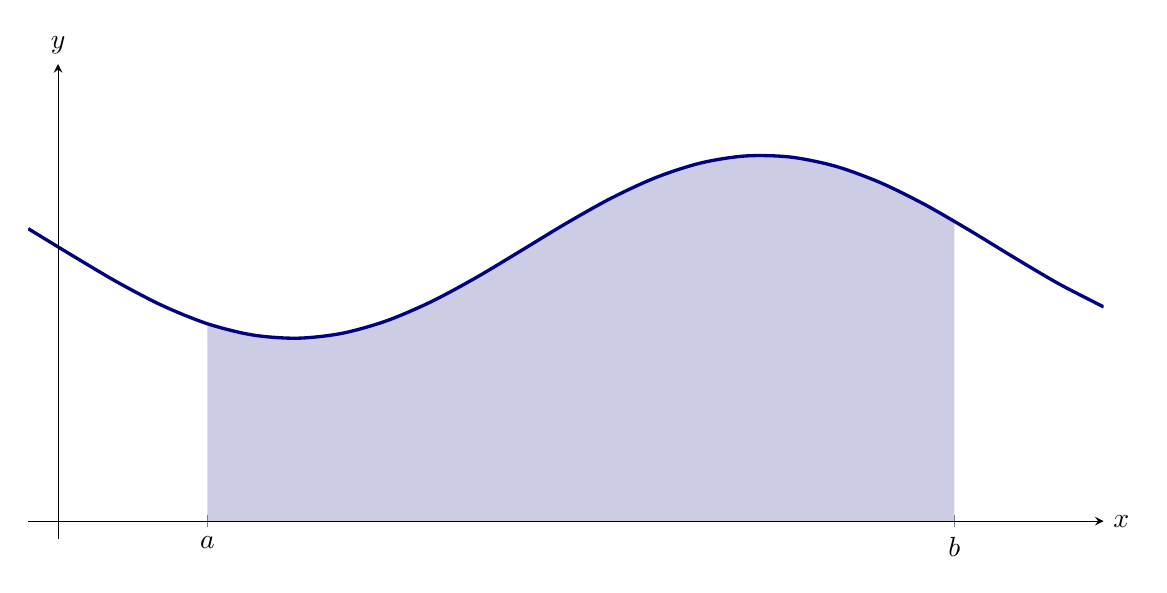
\begin{tikzpicture}[
      declare function = {f(\x) = -sin(deg(\x)) + 3;} ]
	\begin{axis}[
            domain=-.2:7, xmin =-.2,xmax=7,ymax=5,ymin=-.2,
            width=6in,
            height=3in,
            xtick={1,6}, 
            xticklabels={$a$,$b$},
            ytick style={draw=none},
            yticklabels={},
            axis lines=center, xlabel=$x$, ylabel=$y$,
            every axis y label/.style={at=(current axis.above origin),anchor=south},
            every axis x label/.style={at=(current axis.right of origin),anchor=west},
            axis on top,
          ]
          \addplot [draw=none,fill=fillp,domain=1:6, smooth] {f(x)} \closedcycle;
          \addplot [very thick,penColor, smooth] {f(x)};
        \end{axis}
\end{tikzpicture}
\end{image}
One way to do this would be to approximate the area with
rectangles. With one rectangle we get a rough approximation:
\begin{image}
  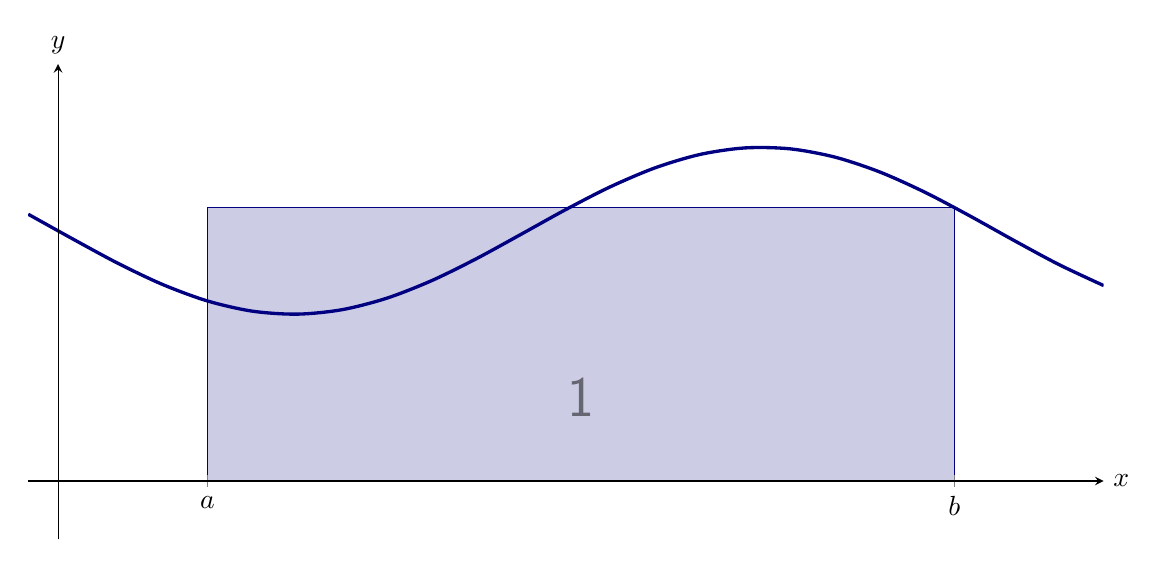
\begin{tikzpicture}[
      declare function = {f(\x) = -sin(deg(\x)) + 3;}]
    \begin{axis}[  
        domain=-.2:7, xmin =-.2,xmax=7,ymax=5,ymin=-.7,
        width=6in,
        height=3in,xtick={1,6},
        xticklabels={$a$,$b$},
        ytick style={draw=none},
        yticklabels={},
        axis lines=center, xlabel=$x$, ylabel=$y$,
        every axis y label/.style={at=(current axis.above origin),anchor=south},
        every axis x label/.style={at=(current axis.right of origin),anchor=west},
        axis on top,
      ]
      \foreach \rectnumber in {1}
               {
                 \addplot [draw=penColor,fill=fillp] plot coordinates
                          {({1+(\rectnumber - 1) * 5},{f(1+\rectnumber * 5)})
                            ({1+(\rectnumber) * 5},{f(1+\rectnumber * 5) })} \closedcycle;
               };
               \addplot [very thick,penColor, smooth] {f(x)};
               \node[fillp!50!black] at (axis cs:3.5,1) {\huge$\mathsf{1}$};
    \end{axis}
  \end{tikzpicture}
\end{image}
Two rectangles might make a better approximation:
\begin{image}
  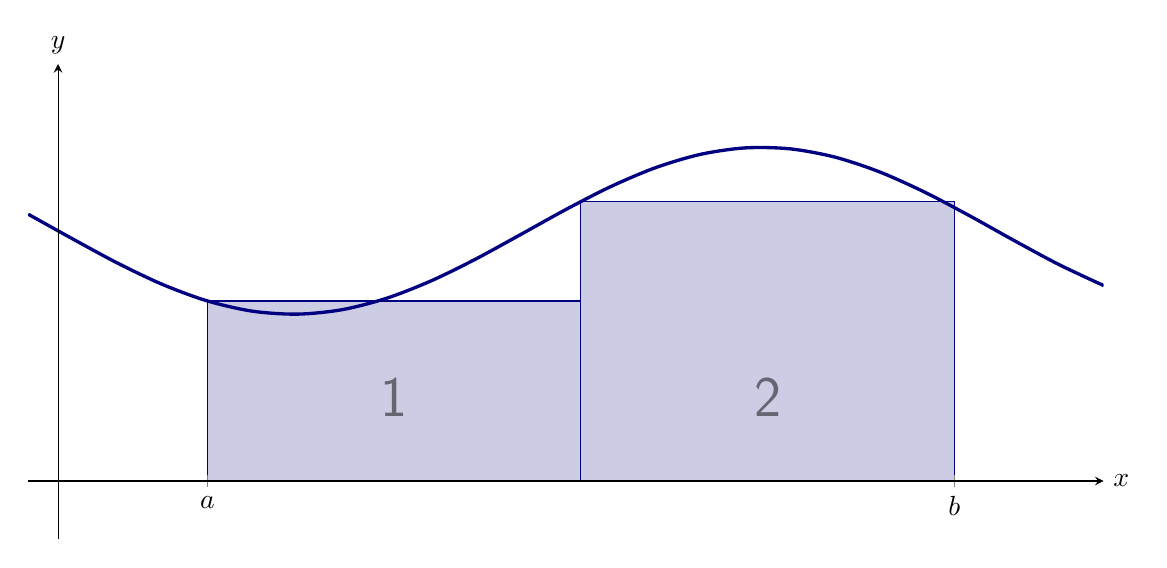
\begin{tikzpicture}[
      declare function = {f(\x) = -sin(deg(\x)) + 3;}]
    \begin{axis}[  
        domain=-.2:7, xmin =-.2,xmax=7,ymax=5,ymin=-.7,
        width=6in,
        height=3in,xtick={1,6},
        xticklabels={$a$,$b$},
        ytick style={draw=none},
        yticklabels={},
        axis lines=center, xlabel=$x$, ylabel=$y$,
        every axis y label/.style={at=(current axis.above origin),anchor=south},
        every axis x label/.style={at=(current axis.right of origin),anchor=west},
        axis on top,
      ]
      \foreach \rectnumber in {1,2}
               {
                 \addplot [draw=penColor,fill=fillp] plot coordinates
                          {({1+(\rectnumber - 1) * 5/2},{f(1+(\rectnumber-1) * 5/2)})
                            ({1+(\rectnumber) * 5/2},{f(1+(\rectnumber-1) * 5/2) })} \closedcycle;
               };
               \addplot [very thick,penColor, smooth] {f(x)};
               \node[fillp!50!black] at (axis cs:2.25,1) {\huge$\mathsf{1}$};
               \node[fillp!50!black] at (axis cs:4.75,1) {\huge$\mathsf{2}$};
    \end{axis}
  \end{tikzpicture}
\end{image}
With even more, we get a closer, and closer, approximation:
\begin{image}
  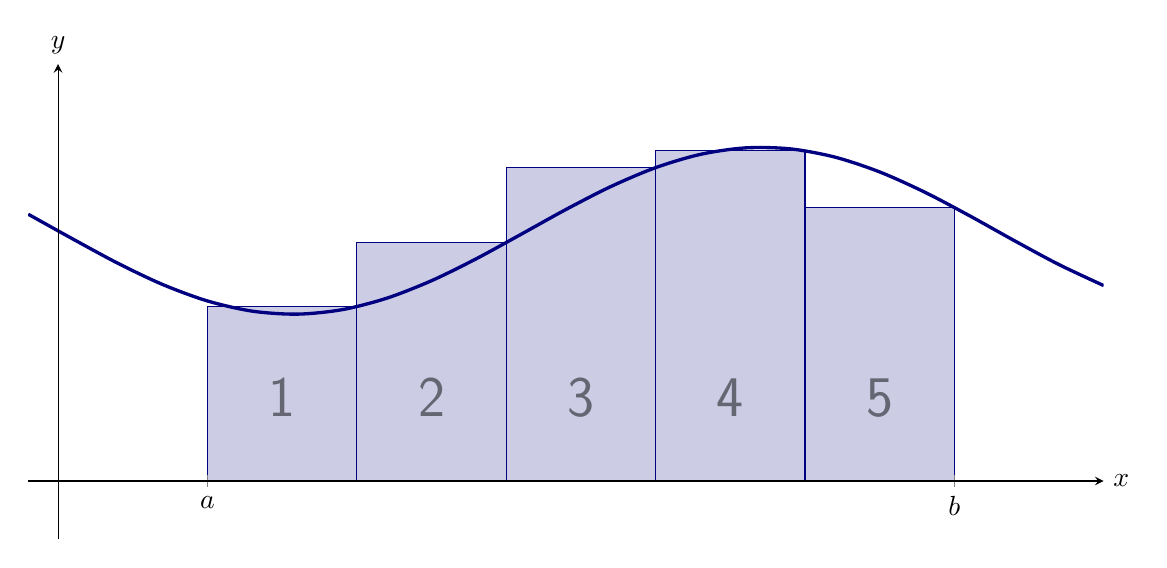
\begin{tikzpicture}[
      declare function = {f(\x) = -sin(deg(\x)) + 3;}]
    \begin{axis}[  
        domain=-.2:7, xmin =-.2,xmax=7,ymax=5,ymin=-.7,
        width=6in,
        height=3in,xtick={1,6},
        xticklabels={$a$,$b$},
        ytick style={draw=none},
        yticklabels={},
        axis lines=center, xlabel=$x$, ylabel=$y$,
        every axis y label/.style={at=(current axis.above origin),anchor=south},
        every axis x label/.style={at=(current axis.right of origin),anchor=west},
        axis on top,
      ]
      \foreach \rectnumber in {1,2,...,5}
               {
                 \addplot [draw=penColor,fill=fillp] plot coordinates
                          {({1+(\rectnumber - 1) * 5/5},{f(1+\rectnumber * 5/5)})
                            ({1+(\rectnumber) * 5/5},{f(1+\rectnumber * 5/5) })} \closedcycle;
               };
               \addplot [very thick,penColor, smooth] {f(x)};
               \node[fillp!50!black] at (axis cs:1.5,1) {\huge$\mathsf{1}$};
               \node[fillp!50!black] at (axis cs:2.5,1) {\huge$\mathsf{2}$};
               \node[fillp!50!black] at (axis cs:3.5,1) {\huge$\mathsf{3}$};
               \node[fillp!50!black] at (axis cs:4.5,1) {\huge$\mathsf{4}$};
               \node[fillp!50!black] at (axis cs:5.5,1) {\huge$\mathsf{5}$};       
    \end{axis}
  \end{tikzpicture}
\end{image}






\begin{definition}
  If we are approximating the area between a curve and the $x$-axis
  on $[a,b]$ with $n$ rectangles of width $\Delta x$, then
  \[
  \Delta x = \frac{b-a}{n}.
  \]
\end{definition}
\begin{image}
  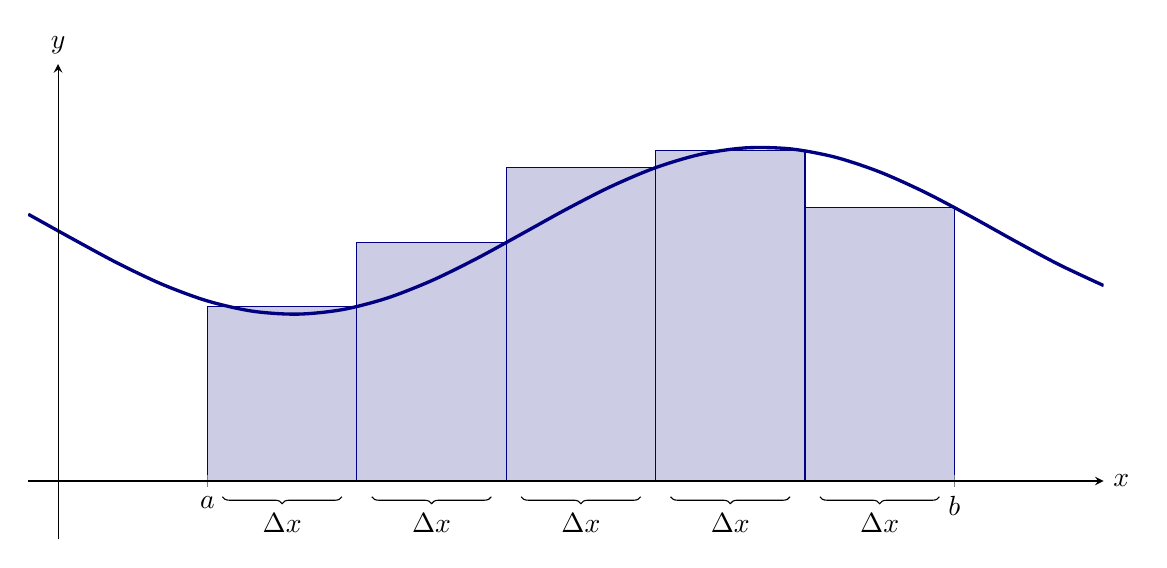
\begin{tikzpicture}[
      declare function = {f(\x) = -sin(deg(\x)) + 3;}]
    \begin{axis}[  
        domain=-.2:7, xmin =-.2,xmax=7,ymax=5,ymin=-.7,
        width=6in,
        height=3in,xtick={1,6},
        xticklabels={$a$,$b$},
        ytick style={draw=none},
        yticklabels={},
        axis lines=center, xlabel=$x$, ylabel=$y$,
        every axis y label/.style={at=(current axis.above origin),anchor=south},
        every axis x label/.style={at=(current axis.right of origin),anchor=west},
        axis on top,
      ]
      \foreach \rectnumber in {1,2,...,5}
               {
                 \addplot [draw=penColor,fill=fillp] plot coordinates
                          {({1+(\rectnumber - 1) * 1},{f(1+\rectnumber * 1)})
                            ({1+(\rectnumber) * 1},{f(1+\rectnumber * 1) })} \closedcycle;

                 \addplot[decoration={brace,mirror,raise=.2cm},decorate,thin] plot coordinates
                          {(\rectnumber+.1,0)
                            (1+\rectnumber-.1,0)};
               };
               \addplot [very thick,penColor, smooth] {f(x)};
               \node at (axis cs:1.5,-.5) {$\Delta x$};
               \node at (axis cs:2.5,-.5) {$\Delta x$};
               \node at (axis cs:3.5,-.5) {$\Delta x$};
               \node at (axis cs:4.5,-.5) {$\Delta x$};
               \node at (axis cs:5.5,-.5) {$\Delta x$};
    \end{axis}
  \end{tikzpicture}
\end{image}
\begin{question}
  Suppose we wanted to approximate area between the curve $y=x^2+1$
  and the $x$-axis on the interval $[-1,1]$, with $8$ rectangles. What is $\Delta x$?
  \begin{prompt}
    \[
    \Delta x = \answer{1/4}
    \]
  \end{prompt}
\end{question}

As we add rectangles, we are more closely approximating the area we are interested in:
\begin{image}
  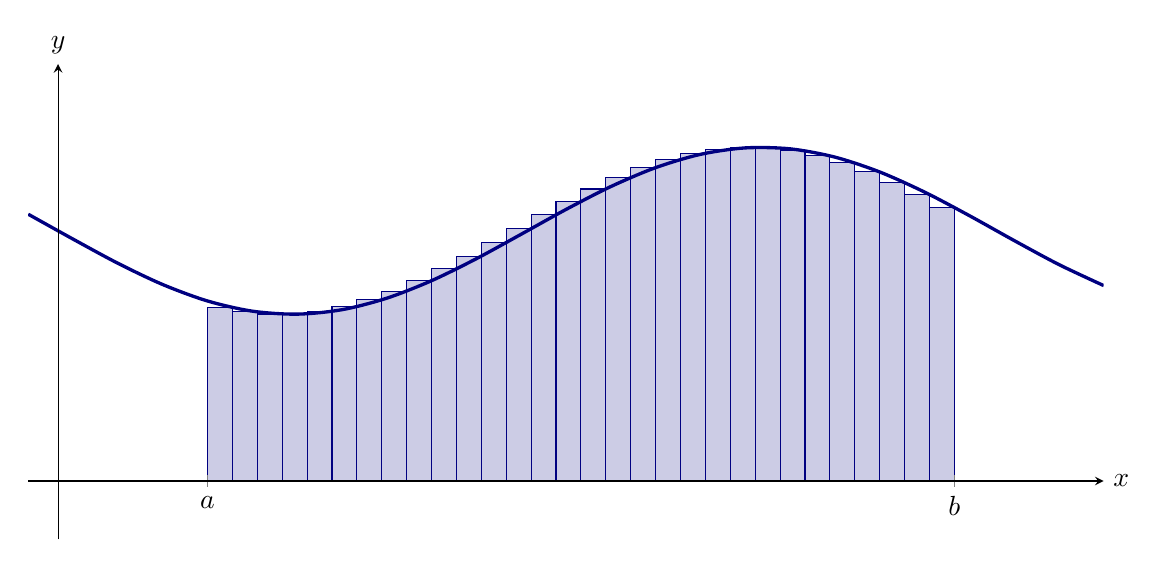
\begin{tikzpicture}[
      declare function = {f(\x) = -sin(deg(\x)) + 3;}]
    \begin{axis}[  
        domain=-.2:7, xmin =-.2,xmax=7,ymax=5,ymin=-.7,
        width=6in,
        height=3in,xtick={1,6},
        xticklabels={$a$,$b$},
        ytick style={draw=none},
        yticklabels={},
        axis lines=center, xlabel=$x$, ylabel=$y$,
        every axis y label/.style={at=(current axis.above origin),anchor=south},
        every axis x label/.style={at=(current axis.right of origin),anchor=west},
        axis on top,
      ]
      \foreach \rectnumber in {1,2,...,30}
               {
                 \addplot [draw=penColor,fill=fillp] plot coordinates
                          {({1+(\rectnumber - 1) * 5/30},{f(1+\rectnumber * 5/30)})
                            ({1+(\rectnumber) * 5/30},{f(1+\rectnumber * 5/30) })} \closedcycle;
               };
               \addplot [very thick,penColor, smooth] {f(x)};
    \end{axis}
  \end{tikzpicture}
\end{image}
%We could find the area exactly if we could compute the limit as the
%width of the rectangles goes to zero and the number of rectangles goes
%to infinity.


Let's setup some notation to help with these calculuations:


\begin{definition}
  When approximating an area with $n$ rectangles, the \dfn{grid
    points}
  \[
  x_0,x_1,x_2,\dots,x_n
  \]
  are the $x$-coordinates that determine the edges of the
  rectangles. In the graph below, we've numbered the rectangles to
  help you see the relation between the indices of the grid points
  and the $k$th rectangle.
\begin{image}
  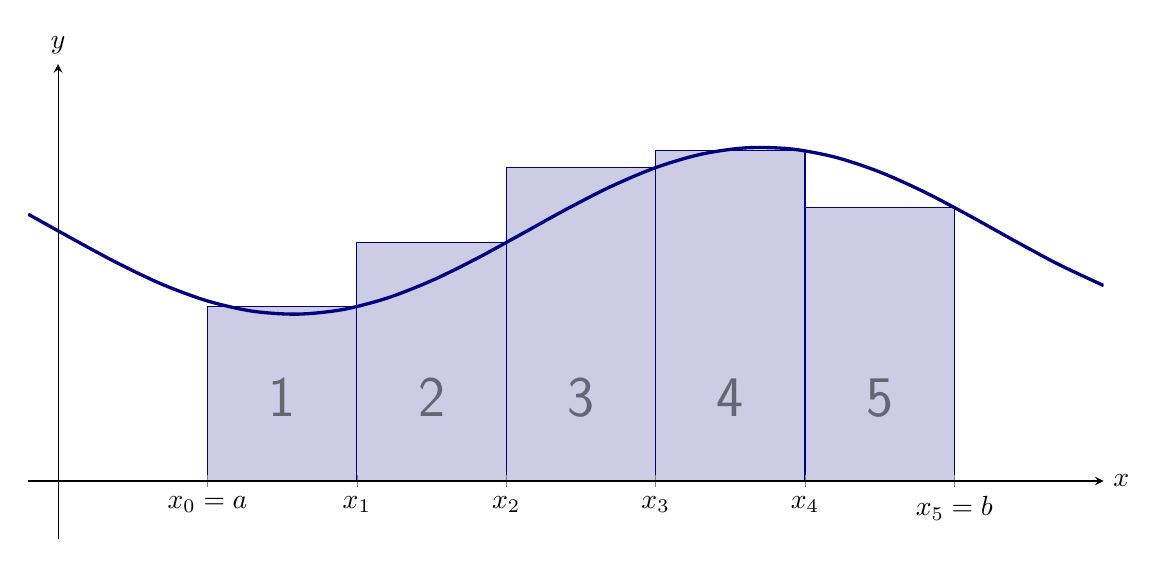
\begin{tikzpicture}[
      declare function = {f(\x) = -sin(deg(\x)) + 3;}]
    \begin{axis}[  
        domain=-.2:7, xmin =-.2,xmax=7,ymax=5,ymin=-.7,
        width=6in,
        height=3in,xtick={1,2,...,6},
        xticklabels={$x_0=a$,$x_1$,$x_2$,$x_3$,$x_4$,$x_5=b$},
        ytick style={draw=none},
        yticklabels={},
        axis lines=center, xlabel=$x$, ylabel=$y$,
        every axis y label/.style={at=(current axis.above origin),anchor=south},
        every axis x label/.style={at=(current axis.right of origin),anchor=west},
        axis on top,
      ]
      \foreach \rectnumber in {1,2,...,5}
               {
                 \addplot [draw=penColor,fill=fillp] plot coordinates
                          {({1+(\rectnumber - 1) * 5/5},{f(1+\rectnumber * 5/5)})
                            ({1+(\rectnumber) * 5/5},{f(1+\rectnumber * 5/5) })} \closedcycle;
               };
               \addplot [very thick,penColor, smooth] {f(x)};
               \node[fillp!50!black] at (axis cs:1.5,1) {\huge$\mathsf{1}$};
               \node[fillp!50!black] at (axis cs:2.5,1) {\huge$\mathsf{2}$};
               \node[fillp!50!black] at (axis cs:3.5,1) {\huge$\mathsf{3}$};
               \node[fillp!50!black] at (axis cs:4.5,1) {\huge$\mathsf{4}$};
               \node[fillp!50!black] at (axis cs:5.5,1) {\huge$\mathsf{5}$};       
    \end{axis}
  \end{tikzpicture}
\end{image}
Note, if we are approximating the area between a curve and the
horizontal axis on $[a,b]$ with $n$ rectangles, then it is always the
case that
\[
x_0=a\qquad\text{and}\qquad x_n = b.
\]
\end{definition}

\begin{question}
  If we are approximating the area between a curve and the horizontal
  axis with $11$ rectangles, how many grid points will we have?
  \begin{hint}
    You can draw it!
  \end{hint}
  \begin{prompt}
    We'll have $\answer{12}$ grid points.
  \end{prompt}
\end{question}







\section{But which set of rectangles?}

If we are going to try and actually use many small rectangles to
compute the area under a curve, we should decide on exactly
\textit{which} rectangles we want to use. We need another definition:

\begin{definition}
  When approximating an area with rectangles, a \dfn{sample point} is
  the $x$-coordinate that determines the relevant height of our
  rectangles. We denote a sample point as:
  \[
  x_k^*
  \]
\end{definition}
The sample point tells us where the rectangles touch the curve.  Here
are three options for sample points that we consider:

\subsection{Rectangles defined by left-endpoints}

We can set the rectangles up so that the left-endpoint touches the
curve.
\begin{image}
  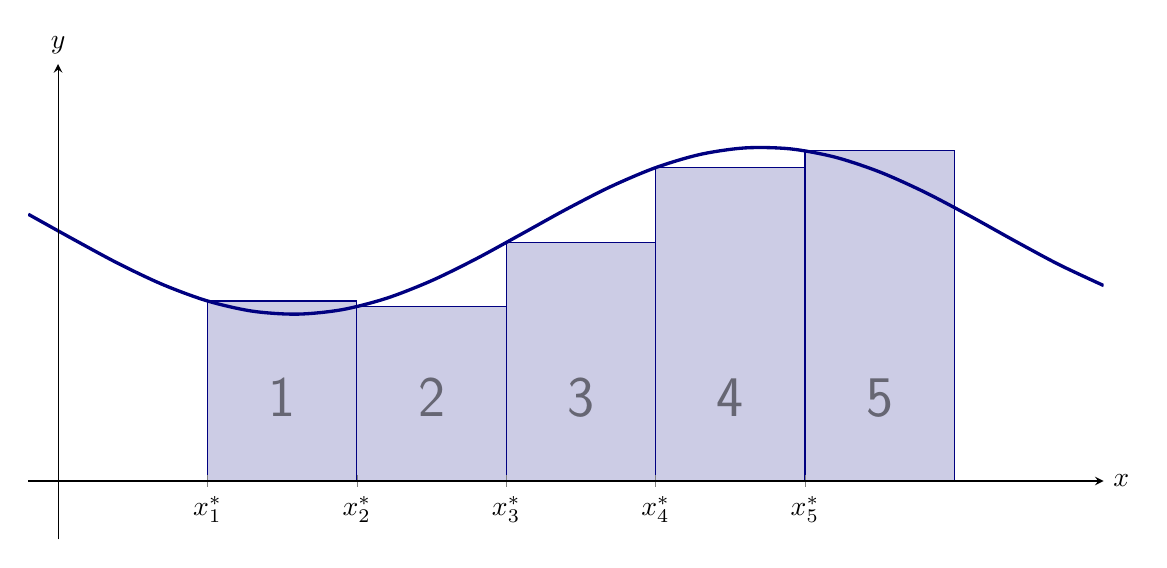
\begin{tikzpicture}[
      declare function = {f(\x) = -sin(deg(\x)) + 3;}]
    \begin{axis}[  
        domain=-.2:7, xmin =-.2,xmax=7,ymax=5,ymin=-.7,
        width=6in,
        height=3in,xtick={1,2,...,5},
        xticklabels={$x_1^*$,$x_2^*$,$x_3^*$,$x_4^*$,$x_5^*$},
        ytick style={draw=none},
        yticklabels={},
        axis lines=center, xlabel=$x$, ylabel=$y$,
        every axis y label/.style={at=(current axis.above origin),anchor=south},
        every axis x label/.style={at=(current axis.right of origin),anchor=west},
        axis on top,
      ]
      \foreach \rectnumber in {1,2,...,5}
               {
                 \addplot [draw=penColor,fill=fillp] plot coordinates
                          {({1+\rectnumber-1) * 5/5},{f(1+(\rectnumber-1) * 5/5)})
                            ({(1+\rectnumber) * 5/5},{f(1+(\rectnumber-1) * 5/5) })} \closedcycle;
               };
               \addplot [very thick,penColor, smooth] {f(x)};
               \node[fillp!50!black] at (axis cs:1.5,1) {\huge$\mathsf{1}$};
               \node[fillp!50!black] at (axis cs:2.5,1) {\huge$\mathsf{2}$};
               \node[fillp!50!black] at (axis cs:3.5,1) {\huge$\mathsf{3}$};
               \node[fillp!50!black] at (axis cs:4.5,1) {\huge$\mathsf{4}$};
               \node[fillp!50!black] at (axis cs:5.5,1) {\huge$\mathsf{5}$}; 
    \end{axis}
  \end{tikzpicture}
\end{image}
In the graph above, the $k$th rectangle's left-endpoint is touching the curve.





\subsection{Rectangles defined by right-endpoints}

We can set the rectangles up so that the right-endpoint touches the
curve.
\begin{image}
  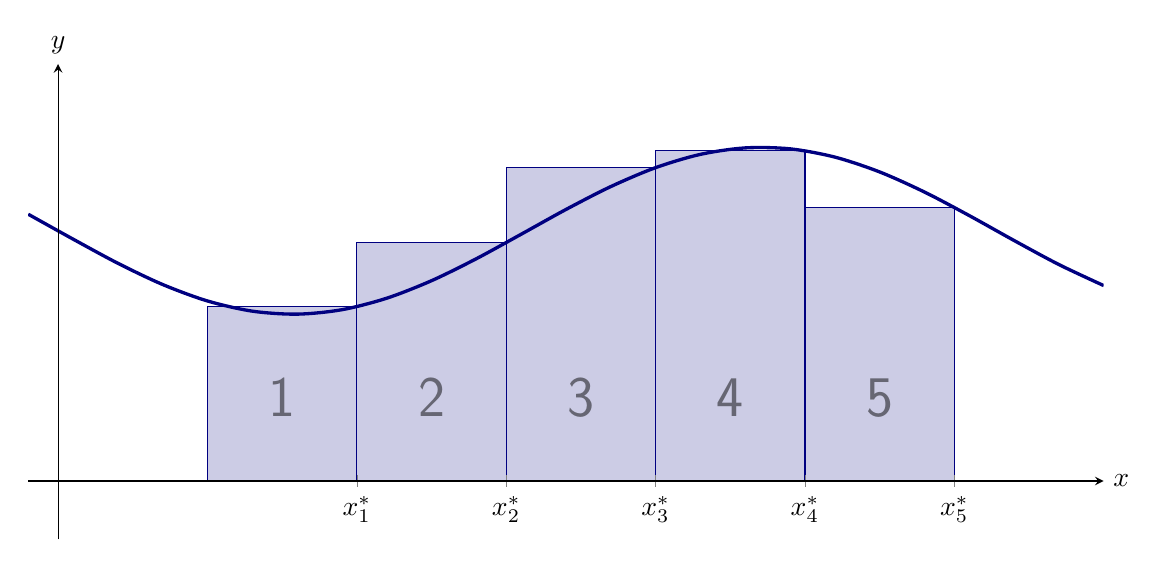
\begin{tikzpicture}[
      declare function = {f(\x) = -sin(deg(\x)) + 3;}]
    \begin{axis}[  
        domain=-.2:7, xmin =-.2,xmax=7,ymax=5,ymin=-.7,
        width=6in,
        height=3in,xtick={2,3,...,6},
        xticklabels={$x_1^*$,$x_2^*$,$x_3^*$,$x_4^*$,$x_5^*$},
        ytick style={draw=none},
        yticklabels={},
        axis lines=center, xlabel=$x$, ylabel=$y$,
        every axis y label/.style={at=(current axis.above origin),anchor=south},
        every axis x label/.style={at=(current axis.right of origin),anchor=west},
        axis on top,
      ]
      \foreach \rectnumber in {1,2,...,5}
               {
                 \addplot [draw=penColor,fill=fillp] plot coordinates
                          {({1+\rectnumber-1) * 5/5},{f(1+(\rectnumber) * 5/5)})
                            ({(1+\rectnumber) * 5/5},{f(1+(\rectnumber) * 5/5) })} \closedcycle;
               };
               \addplot [very thick,penColor, smooth] {f(x)};
               \node[fillp!50!black] at (axis cs:1.5,1) {\huge$\mathsf{1}$};
               \node[fillp!50!black] at (axis cs:2.5,1) {\huge$\mathsf{2}$};
               \node[fillp!50!black] at (axis cs:3.5,1) {\huge$\mathsf{3}$};
               \node[fillp!50!black] at (axis cs:4.5,1) {\huge$\mathsf{4}$};
               \node[fillp!50!black] at (axis cs:5.5,1) {\huge$\mathsf{5}$}; 
    \end{axis}
  \end{tikzpicture}
\end{image}
In the graph above, the $k$th rectangle's right-endpoint is touching the curve.


\subsection{Rectangles defined by midpoints}

We can set the rectangles up so that the midpoint of one of the
horizontal sides touches the curve.
\begin{image}
  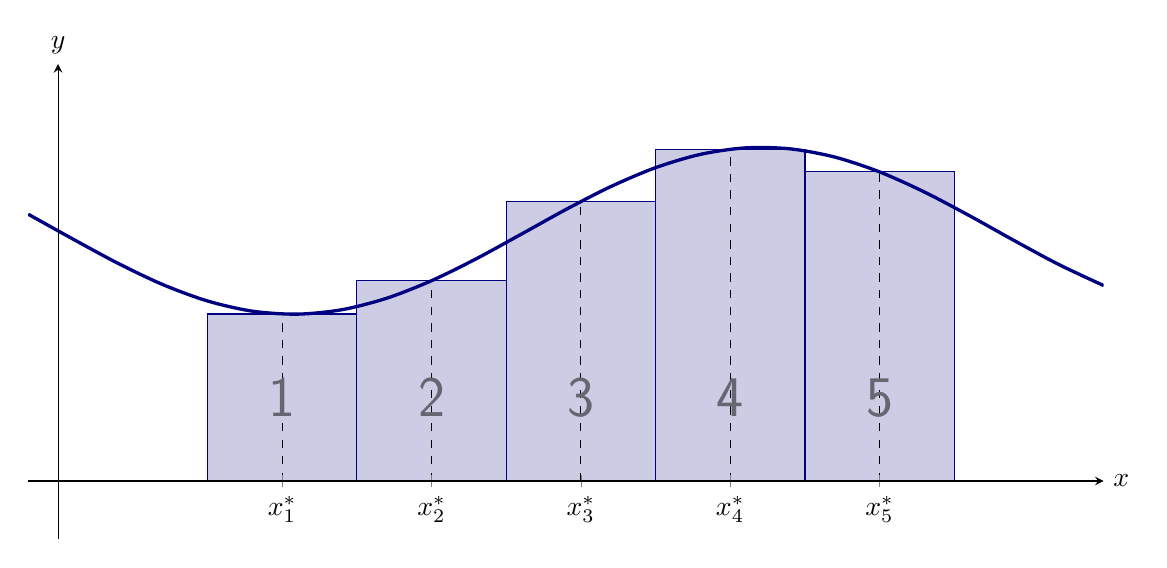
\begin{tikzpicture}[
      declare function = {f(\x) = -sin(deg(\x)) + 3;}]
    \begin{axis}[  
        domain=-.2:7, xmin =-.2,xmax=7,ymax=5,ymin=-.7,
        width=6in,
        height=3in,xtick={1.5,2.5,...,5.5},
        xticklabels={$x_1^*$,$x_2^*$,$x_3^*$,$x_4^*$,$x_5^*$},
        ytick style={draw=none},
        yticklabels={},
        axis lines=center, xlabel=$x$, ylabel=$y$,
        every axis y label/.style={at=(current axis.above origin),anchor=south},
        every axis x label/.style={at=(current axis.right of origin),anchor=west},
        axis on top,
      ]
      \foreach \rectnumber in {1,2,...,5}
               {
                 \addplot [draw=penColor,fill=fillp] plot coordinates
                          {({1+\rectnumber-1) * 5/5},{f(1+(\rectnumber-.5) * 5/5)})
                            ({(1+\rectnumber) * 5/5},{f(1+(\rectnumber-.5) * 5/5) })} \closedcycle;
                 \addplot [draw=black,dashed] plot coordinates
                                   {({1+\rectnumber-.5) * 5/5},{0 * 5/5)})
                            ({(1+\rectnumber-.5) * 5/5},{f(1+(\rectnumber-.5) * 5/5) })};
               };
               \addplot [very thick,penColor, smooth] {f(x)};
               \node[fillp!50!black] at (axis cs:1.5,1) {\huge$\mathsf{1}$};
               \node[fillp!50!black] at (axis cs:2.5,1) {\huge$\mathsf{2}$};
               \node[fillp!50!black] at (axis cs:3.5,1) {\huge$\mathsf{3}$};
               \node[fillp!50!black] at (axis cs:4.5,1) {\huge$\mathsf{4}$};
               \node[fillp!50!black] at (axis cs:5.5,1) {\huge$\mathsf{5}$}; 
    \end{axis}
  \end{tikzpicture}
\end{image}
In the graph above, the midpoint of the horizontal side of the $k$th
rectangle is touching the curve.


%% \begin{question}
%%   Which approximation is most accurate?
%%   \begin{multipleChoice}
%%     \choice{Approximations with left-endpoints.}
%%     \choice{Approximations with right-endpoints.}
%%     \choice{Approximations with midpoints.}
%%     \choice[correct]{It depends on the function.}
%%   \end{multipleChoice}
%% \end{question}



\section{Riemann sums and approximating area}

Once we know how to identify our rectangles, we can compute some
approximate areas. If we are approximating area with $n$ rectangles, then 
%\begin{align*}
%  \text{Area} &\approx \sum_{k=1}^n (\text{height of $k$th rectangle})\times(\text{width of $k$th rectangle}) \\
%  &=\sum_{k=1}^n  f(x_k^*)\Delta x \\
%  &=  f(x_1^*)\Delta x +  f(x_2^*)\Delta x +   f(x_3^*)\Delta x + \dots +   %f(x_n^*)\Delta x. 
%\end{align*}
the area of the $k$th rectangle (for $k$ between $1$ and $n$) is given by:
\[ (\text{height of $k$th rectangle}) \times (\text{width of $k$th rectangle})
	= f(x_k^*) \Delta x \] 
The area of the region is approximately:
\[  \text{Area} \approx  
	f(x_1^*)\Delta x +  f(x_2^*)\Delta x +   f(x_3^*)\Delta x + \dots +   f(x_n^*)\Delta x.  \]
\begin{definition}
  A sum of the form:
%  \[
%  \sum_{k=1}^n  f(x_k^*)\Delta x  = f(x_1^*)\Delta x +  f(x_2^*)\Delta x + \dots %+   f(x_n^*)\Delta x
%  \]
  \[ f(x_1^*)\Delta x +  f(x_2^*)\Delta x + \dots +   f(x_n^*)\Delta x \]
  is called a \dfn{Riemann sum}, pronounced ``ree-mahn'' sum. 
\end{definition}

A Riemann sum computes an approximation of the area between a curve
and the $x$-axis on the interval $[a,b]$. It can be defined several
different ways. In our class, it will be defined via left-endpoints,
right-endpoints, or midpoints. Here we see the explicit connection
between a Riemann sum defined by left-endpoints and the area between a curve
and the $x$-axis on the interval $[a,b]$:
\begin{image}
  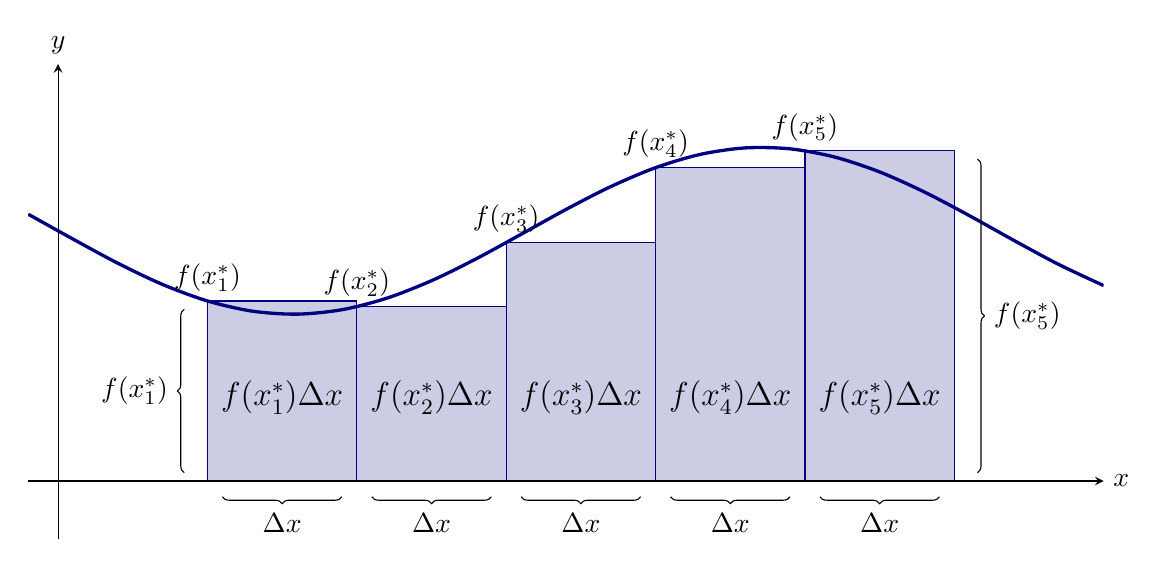
\begin{tikzpicture}[
      declare function = {f(\x) = -sin(deg(\x)) + 3;}]
    \begin{axis}[  
        domain=-.2:7, xmin =-.2,xmax=7,ymax=5,ymin=-.7,
        width=6in,
        height=3in,
        xtick style={draw=none},
        xticklabels={},
        ytick style={draw=none},
        yticklabels={},
        axis lines=center, xlabel=$x$, ylabel=$y$,
        every axis y label/.style={at=(current axis.above origin),anchor=south},
        every axis x label/.style={at=(current axis.right of origin),anchor=west},
        axis on top,
      ]
      \foreach \rectnumber in {1,2,...,5}
               {
                 \addplot [draw=penColor,fill=fillp] plot coordinates
                          {({1+\rectnumber-1) * 5/5},{f(1+(\rectnumber-1) * 5/5)})
                            ({(1+\rectnumber) * 5/5},{f(1+(\rectnumber-1) * 5/5) })} \closedcycle;
                 \addplot[decoration={brace,mirror,raise=.2cm},decorate,thin] plot coordinates
                          {(\rectnumber+.1,0)
                            (1+\rectnumber-.1,0)};
               };
               \addplot [very thick,penColor, smooth] {f(x)};
               \addplot[decoration={brace,raise=.2cm},decorate,thin] plot coordinates
                       {(.95,.1) (.95,{f(1)-.1})};
               \addplot[decoration={brace,mirror,raise=.2cm},decorate,thin] plot coordinates
                       {(6.05,.1) (6.05,{f(5)-.1})};
               \node at (axis cs:1.5,-.5) {$\Delta x$};
               \node at (axis cs:2.5,-.5) {$\Delta x$};
               \node at (axis cs:3.5,-.5) {$\Delta x$};
               \node at (axis cs:4.5,-.5) {$\Delta x$};
               \node at (axis cs:5.5,-.5) {$\Delta x$};

               \node at (axis cs:1.5,1) {\large$f(x_1^*)\Delta x$};
               \node at (axis cs:2.5,1) {\large$f(x_2^*)\Delta x$};
               \node at (axis cs:3.5,1) {\large$f(x_3^*)\Delta x$};
               \node at (axis cs:4.5,1) {\large$f(x_4^*)\Delta x$};
               \node at (axis cs:5.5,1) {\large$f(x_5^*)\Delta x$};

               \node[anchor=east] at (axis cs:.8,{f(1)/2}) {$f(x_1^*)$};
               \node[anchor=west] at (axis cs:6.2,{f(5)/2}) {$f(x_5^*)$};
               
               \node[anchor=south] at (axis cs:1,{f(1)}) {$f(x_1^*)$};
               \node[anchor=south] at (axis cs:2,{f(2)}) {$f(x_2^*)$};
               \node[anchor=south] at (axis cs:3,{f(3)}) {$f(x_3^*)$};
               \node[anchor=south] at (axis cs:4,{f(4)}) {$f(x_4^*)$};
               \node[anchor=south] at (axis cs:5,{f(5)}) {$f(x_5^*)$};
    \end{axis}
  \end{tikzpicture}
\end{image}
and here is the associated Riemann sum
\[
%\sum_{k=1}^5  f(x_k^*)\Delta x  = 
f(x_1^*)\Delta x +  f(x_2^*)\Delta x +   f(x_3^*)\Delta x + f(x_4^*)\Delta x + f(x_5^*)\Delta x.
\]



\subsection{Left Riemann sums}

\begin{example}
  Consider $f(x) = x^3/8-x+2$. Approximate the area between $f$ and
  the $x$-axis on the interval $[-1,3]$ using a left-endpoint Riemann
  sum with $n=5$ rectangles.
  
  \begin{explanation}
    First note that the width of each rectangle is
    \[
    \Delta x = \frac{3-(-1)}{5} = \answer[given]{4/5}.
    \]
    The grid points define the edges of the rectangle and are seen below:
\begin{image}
  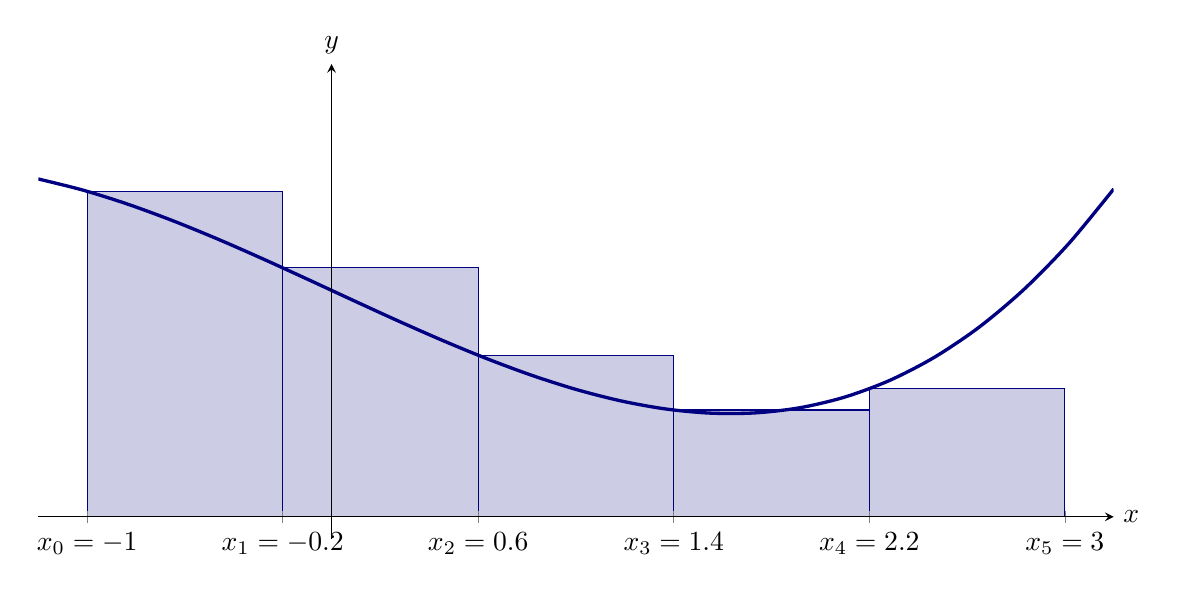
\begin{tikzpicture}[
      declare function = {f(\x) = pow(\x/2,3) -\x+2;}
      ]
	\begin{axis}[
            domain=-1.2:3.2, xmin =-1.2,xmax=3.2,ymax=4,ymin=-.2,
            width=6in,
            height=3in,
            axis lines=center, xlabel=$x$, ylabel=$y$,
            every axis y label/.style={at=(current axis.above origin),anchor=south},
            every axis x label/.style={at=(current axis.right of origin),anchor=west},
            xtick={-1,-.2,...,3.8},
            xticklabels={$x_0=-1$,$x_1=-0.2$,$x_2=0.6$,$x_3=1.4$,$x_4=2.2$,$x_5=3$},
            ytick style={draw=none},
            yticklabels={},
            axis on top,
          ]
          \foreach \rectnumber in {1,2,...,5}
                   {
                     \addplot [draw=penColor,fill=fillp] plot coordinates
                              {({-1+(\rectnumber-1) * 4/5},{f(-1+(\rectnumber-1) * 4/5)})
                                ({-1+(\rectnumber) * 4/5},{f(-1+(\rectnumber-1) * 4/5) })} \closedcycle;
               };
                   \addplot [very thick,penColor, smooth] {f(x)};
        \end{axis}
\end{tikzpicture}
\end{image}
On the other hand, the sample points identify which endpoints we use:
\begin{image}
  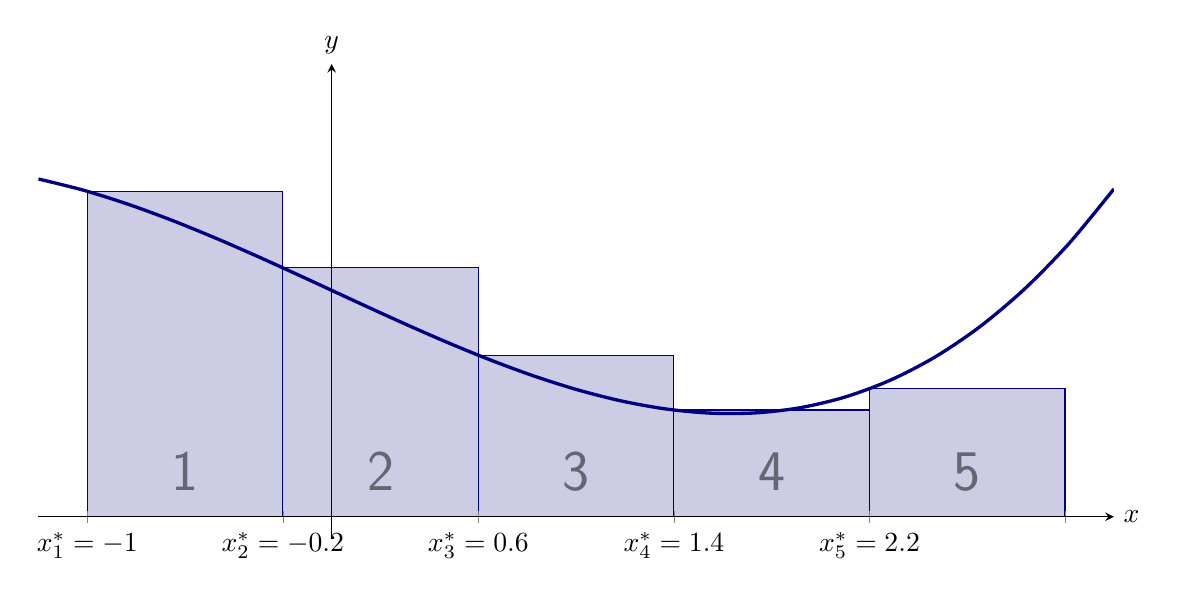
\begin{tikzpicture}[
      declare function = {f(\x) = pow(\x/2,3) -\x+2;}
      ]
	\begin{axis}[
            domain=-1.2:3.2, xmin =-1.2,xmax=3.2,ymax=4,ymin=-.2,
            width=6in,
            height=3in,
            axis lines=center, xlabel=$x$, ylabel=$y$,
            every axis y label/.style={at=(current axis.above origin),anchor=south},
            every axis x label/.style={at=(current axis.right of origin),anchor=west},
            xtick={-1,-.2,...,3},
            xticklabels={$x_1^*=-1$,$x_2^*=-0.2$,$x_3^*=0.6$,$x_4^*=1.4$,$x_5^*=2.2$},
            ytick style={draw=none},
            yticklabels={},
            axis on top,
          ]
          \foreach \rectnumber in {1,2,...,5}
                   {
                     \addplot [draw=penColor,fill=fillp] plot coordinates
                              {({-1+(\rectnumber-1) * 4/5},{f(-1+(\rectnumber-1) * 4/5)})
                                ({-1+(\rectnumber) * 4/5},{f(-1+(\rectnumber-1) * 4/5) })} \closedcycle;
               };
                   \addplot [very thick,penColor, smooth] {f(x)};
                   \node[fillp!50!black] at (axis cs:-.6,.4) {\huge$\mathsf{1}$};
               \node[fillp!50!black] at (axis cs:.2,.4) {\huge$\mathsf{2}$};
               \node[fillp!50!black] at (axis cs:1,.4) {\huge$\mathsf{3}$};
               \node[fillp!50!black] at (axis cs:1.8,.4) {\huge$\mathsf{4}$};
               \node[fillp!50!black] at (axis cs:2.6,.4) {\huge$\mathsf{5}$}; 
        \end{axis}
\end{tikzpicture}
\end{image}
It is helpful to collect all of this data into a table:
\[
\begin{array}{c|c|c|c}
  k &  x_k & x^*_k & f(x^*_k) \\ \hline
  0 & \answer[given]{-1}   & \text{NA} & \text{NA}  \\
  1 & \answer[given]{-0.2} & \answer[given]{-1}        &   \answer[given]{2.875}     \\
  2 & \answer[given]{0.6}  & \answer[given]{-0.2}      & \answer[given]{2.199}   \\
  3 & \answer[given]{1.4}  & \answer[given]{0.6}       & \answer[given]{1.427}    \\
  4 & \answer[given]{2.2}  & \answer[given]{1.4}       & \answer[given]{0.943}   \\
  5 & \answer[given]{3}    & \answer[given]{2.2}      & \answer[given]{1.131}        \\
\end{array}
\]
Now we may write a left Riemann sum and approximate the area
\[
f(x_1^*)\Delta x +  f(x_2^*)\Delta x +   f(x_3^*)\Delta x +f(x_4^*)\Delta x+   f(x_5^*)\Delta x,
\]
which evaluates to
\begin{align*}
  = 2.875 \cdot (4/5) &+ 2.199  \cdot(4/5) + 1.427  \cdot(4/5)\\
  &+ 0.943  \cdot(4/5) + 1.131  \cdot(4/5)
\end{align*}
and we find
\[
  = \answer[given]{6.86}.
\]
  \end{explanation}
\end{example}


\subsection{Right Riemann sums}


\begin{example}
  Consider $f(x) = x^3/8-x+2$. Approximate the area between $f$ and
  the $x$-axis on the interval $[-1,3]$ using a right-endpoint Riemann
  sum with $n=5$ rectangles.
  
  \begin{explanation}
    First note that the width of each rectangle is
    \[
    \Delta x = \frac{3-(-1)}{5} = \answer[given]{4/5}.
    \]
    The grid points define the edges of the rectangle and are seen below:
\begin{image}
  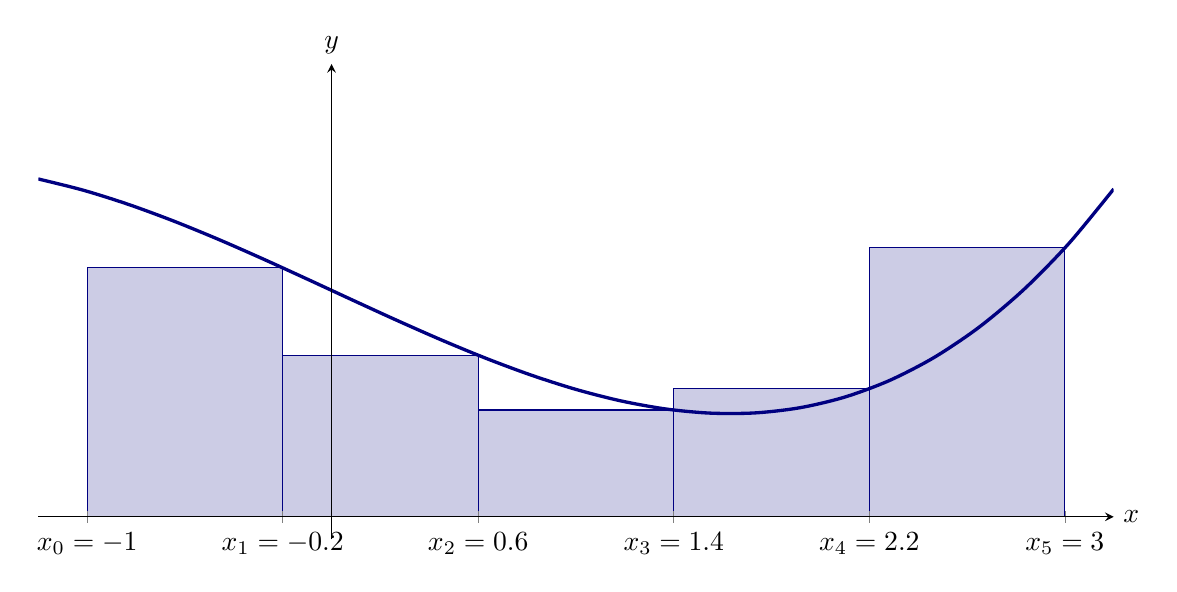
\begin{tikzpicture}[
      declare function = {f(\x) = pow(\x/2,3) -\x+2;}
      ]
	\begin{axis}[
            domain=-1.2:3.2, xmin =-1.2,xmax=3.2,ymax=4,ymin=-.2,
            width=6in,
            height=3in,
            axis lines=center, xlabel=$x$, ylabel=$y$,
            every axis y label/.style={at=(current axis.above origin),anchor=south},
            every axis x label/.style={at=(current axis.right of origin),anchor=west},
            xtick={-1,-.2,...,3.8},
            xticklabels={$x_0=-1$,$x_1=-0.2$,$x_2=0.6$,$x_3=1.4$,$x_4=2.2$,$x_5=3$},
            ytick style={draw=none},
            yticklabels={},
            axis on top,
          ]
          \foreach \rectnumber in {1,2,...,5}
                   {
                     \addplot [draw=penColor,fill=fillp] plot coordinates
                              {({-1+(\rectnumber-1) * 4/5},{f(-1+(\rectnumber) * 4/5)})
                                ({-1+(\rectnumber) * 4/5},{f(-1+(\rectnumber) * 4/5) })} \closedcycle;
               };
                   \addplot [very thick,penColor, smooth] {f(x)};
        \end{axis}
\end{tikzpicture}
\end{image}
On the other hand, the sample points identify which endpoints we use:
\begin{image}
  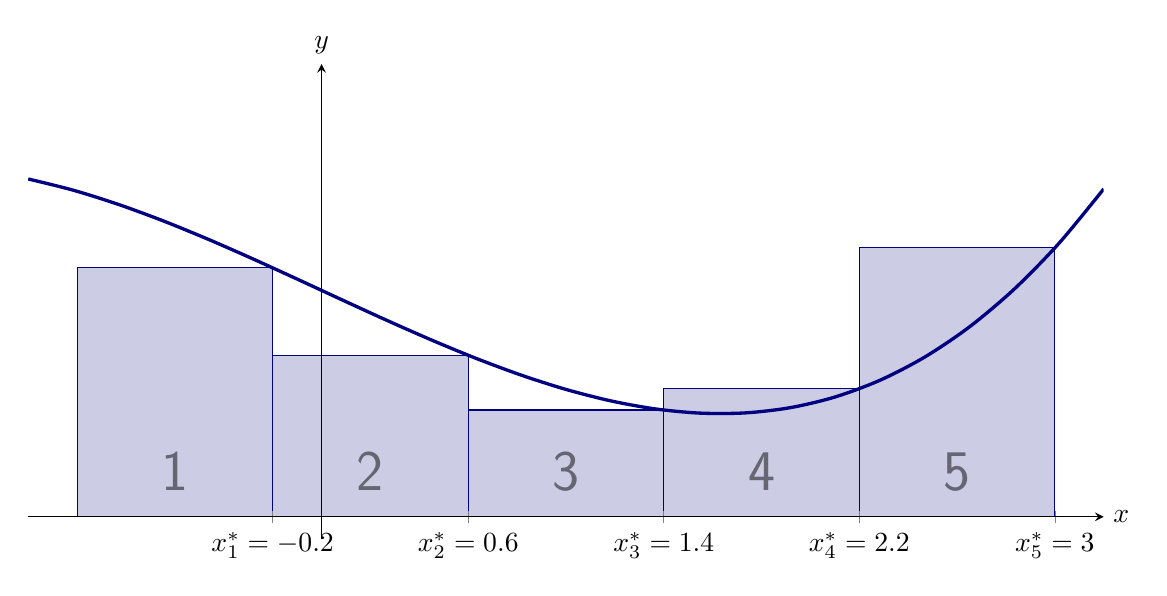
\begin{tikzpicture}[
      declare function = {f(\x) = pow(\x/2,3) -\x+2;}
      ]
	\begin{axis}[
            domain=-1.2:3.2, xmin =-1.2,xmax=3.2,ymax=4,ymin=-.2,
            width=6in,
            height=3in,
            axis lines=center, xlabel=$x$, ylabel=$y$,
            every axis y label/.style={at=(current axis.above origin),anchor=south},
            every axis x label/.style={at=(current axis.right of origin),anchor=west},
            xtick={-.2,.6,1.4,2.2,3},
            xticklabels={$x_1^*=-0.2$,$x_2^*=0.6$,$x_3^*=1.4$,$x_4^*=2.2$,$x_5^*=3$},
            ytick style={draw=none},
            yticklabels={},
            axis on top,
          ]
          \foreach \rectnumber in {1,2,...,5}
                   {
                     \addplot [draw=penColor,fill=fillp] plot coordinates
                              {({-1+(\rectnumber-1) * 4/5},{f(-1+(\rectnumber) * 4/5)})
                                ({-1+(\rectnumber) * 4/5},{f(-1+(\rectnumber) * 4/5) })} \closedcycle;
               };
                   \addplot [very thick,penColor, smooth] {f(x)};
                   \node[fillp!50!black] at (axis cs:-.6,.4) {\huge$\mathsf{1}$};
               \node[fillp!50!black] at (axis cs:.2,.4) {\huge$\mathsf{2}$};
               \node[fillp!50!black] at (axis cs:1,.4) {\huge$\mathsf{3}$};
               \node[fillp!50!black] at (axis cs:1.8,.4) {\huge$\mathsf{4}$};
               \node[fillp!50!black] at (axis cs:2.6,.4) {\huge$\mathsf{5}$}; 
        \end{axis}
\end{tikzpicture}
\end{image}
It is helpful to collect all of this data into a table:
\[
\begin{array}{c|c|c|c}
  k &  x_k & x^*_k & f(x^*_k) \\ \hline
  0 & \answer[given]{-1}   & \text{NA} & \text{NA}  \\
  1 & \answer[given]{-0.2} & \answer[given]{-0.2}      & \answer[given]{2.199}   \\
  2 & \answer[given]{0.6}  & \answer[given]{0.6}       & \answer[given]{1.427}   \\
  3 & \answer[given]{1.4}  & \answer[given]{1.4}       & \answer[given]{0.943}   \\
  4 & \answer[given]{2.2}  & \answer[given]{2.2}       & \answer[given]{1.131}   \\
  5 & \answer[given]{3}    & \answer[given]{3}         & \answer[given]{2.375}   \\
\end{array}
\]
Now we may write a right Riemann sum and approximate the area
\[
f(x_1^*)\Delta x +  f(x_2^*)\Delta x +   f(x_3^*)\Delta x +f(x_4^*)\Delta x+   f(x_5^*)\Delta x,
\]
which evaluates to
\begin{align*}
  = 2.199 \cdot (4/5) &+ 1.427  \cdot(4/5) + 0.943  \cdot(4/5)\\
  &+ 1.131  \cdot(4/5) + 2.375  \cdot(4/5)
\end{align*}
and we find
\[
  = \answer[given]{6.46}.
\]
  \end{explanation}
\end{example}




\subsection{Midpoint Riemann sums}

\begin{example}
  Consider $f(x) = x^3/8-x+2$. Approximate the area between $f$ and
  the $x$-axis on the interval $[-1,3]$ using a midpoint Riemann
  sum with $n=5$ rectangles.
  
  \begin{explanation}
    First note that the width of each rectangle is
    \[
    \Delta x = \frac{3-(-1)}{5} = \answer[given]{4/5}.
    \]
    The grid points define the edges of the rectangle and are seen below:
\begin{image}
  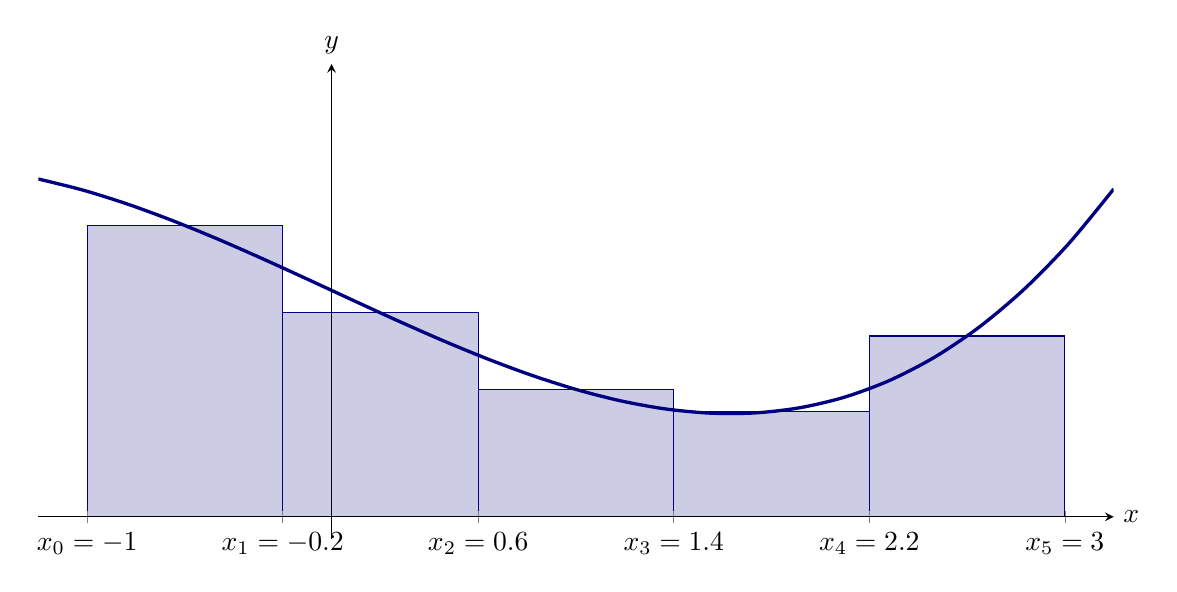
\begin{tikzpicture}[
      declare function = {f(\x) = pow(\x/2,3) -\x+2;}
      ]
	\begin{axis}[
            domain=-1.2:3.2, xmin =-1.2,xmax=3.2,ymax=4,ymin=-.2,
            width=6in,
            height=3in,
            axis lines=center, xlabel=$x$, ylabel=$y$,
            every axis y label/.style={at=(current axis.above origin),anchor=south},
            every axis x label/.style={at=(current axis.right of origin),anchor=west},
            xtick={-1,-.2,...,3.8},
            xticklabels={$x_0=-1$,$x_1=-0.2$,$x_2=0.6$,$x_3=1.4$,$x_4=2.2$,$x_5=3$},
            ytick style={draw=none},
            yticklabels={},
            axis on top,
          ]
          \foreach \rectnumber in {1,2,...,5}
                   {
                     \addplot [draw=penColor,fill=fillp] plot coordinates
                              {({-1+(\rectnumber-1) * 4/5},{f(-1+(\rectnumber-.5) * 4/5)})
                                ({-1+(\rectnumber) * 4/5},{f(-1+(\rectnumber-.5) * 4/5) })} \closedcycle;
               };
                   \addplot [very thick,penColor, smooth] {f(x)};
        \end{axis}
\end{tikzpicture}
\end{image}
On the other hand, the sample points identify which endpoints we use:
\begin{image}
  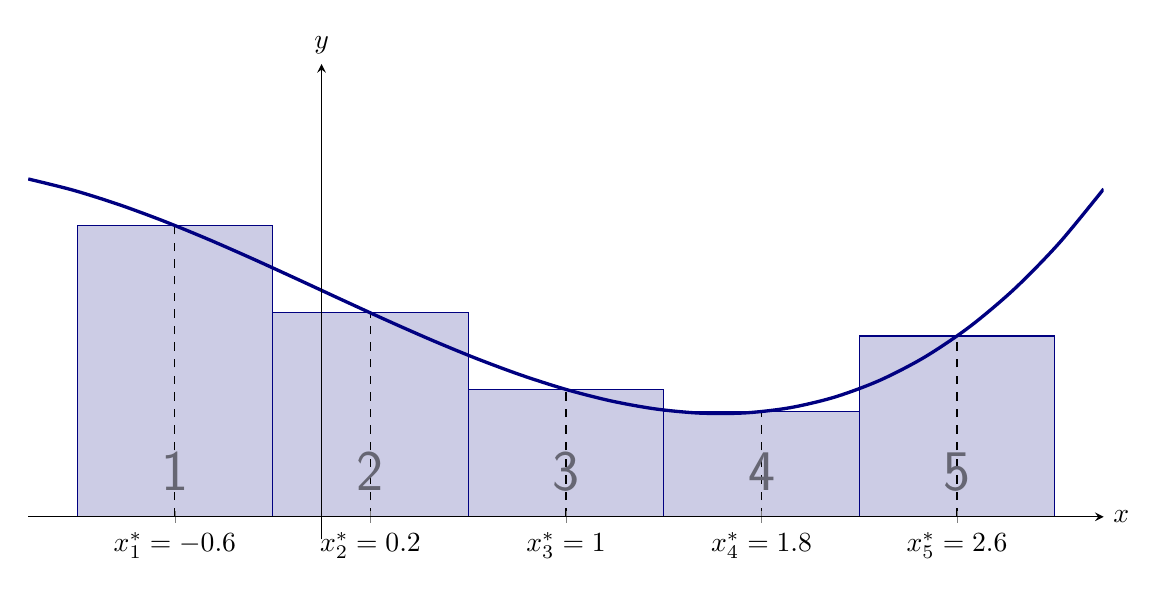
\begin{tikzpicture}[
      declare function = {f(\x) = pow(\x/2,3) -\x+2;}
      ]
	\begin{axis}[
            domain=-1.2:3.2, xmin =-1.2,xmax=3.2,ymax=4,ymin=-.2,
            width=6in,
            height=3in,
            axis lines=center, xlabel=$x$, ylabel=$y$,
            every axis y label/.style={at=(current axis.above origin),anchor=south},
            every axis x label/.style={at=(current axis.right of origin),anchor=west},
            xtick={-.6,.2,1,1.8,2.6},
            xticklabels={$x_1^*=-0.6$,$x_2^*=0.2$,$x_3^*=1$,$x_4^*=1.8$,$x_5^*=2.6$},
            ytick style={draw=none},
            yticklabels={},
            axis on top,
          ]
          \foreach \rectnumber in {1,2,...,5}
                   {
                     \addplot [draw=penColor,fill=fillp] plot coordinates
                              {({-1+(\rectnumber-1) * 4/5},{f(-1+(\rectnumber-.5) * 4/5)})
                                ({-1+(\rectnumber) * 4/5},{f(-1+(\rectnumber-.5) * 4/5) })} \closedcycle;
                     \addplot [draw=black,dashed] plot coordinates
                                   {({-1+(\rectnumber-.5) * 4/5},{0 * 4/5)})
                            ({(-1+(\rectnumber-.5) * 4/5},{f(-1+(\rectnumber-.5) * 4/5) })};
               };
                   \addplot [very thick,penColor, smooth] {f(x)};
                   \node[fillp!50!black] at (axis cs:-.6,.4) {\huge$\mathsf{1}$};
               \node[fillp!50!black] at (axis cs:.2,.4) {\huge$\mathsf{2}$};
               \node[fillp!50!black] at (axis cs:1,.4) {\huge$\mathsf{3}$};
               \node[fillp!50!black] at (axis cs:1.8,.4) {\huge$\mathsf{4}$};
               \node[fillp!50!black] at (axis cs:2.6,.4) {\huge$\mathsf{5}$}; 
        \end{axis}
\end{tikzpicture}
\end{image}
It is helpful to collect all of this data into a table:
\[
\begin{array}{c|c|c|c}
  k &  x_k & x^*_k & f(x^*_k) \\ \hline
  0 & \answer[given]{-1}   & \text{NA} & \text{NA}  \\
  1 & \answer[given]{-0.2} & \answer[given]{-0.6}    & \answer[given]{2.573}   \\
  2 & \answer[given]{0.6}  & \answer[given]{0.2}     & \answer[given]{1.801}   \\
  3 & \answer[given]{1.4}  & \answer[given]{1}       & \answer[given]{1.125}   \\
  4 & \answer[given]{2.2}  & \answer[given]{1.8}     & \answer[given]{0.929}   \\
  5 & \answer[given]{3}    & \answer[given]{2.6}     & \answer[given]{1.597}   \\
\end{array}
\]
Now we may write a midpoint Riemann sum and approximate the area
\[
f(x_1^*)\Delta x + f(x_2^*)\Delta x + f(x_3^*)\Delta x+ f(x_4^*)\Delta x + f(x_5^*)\Delta x,
\]
which evaluates to
\begin{align*}
  = 2.573 \cdot (4/5) &+ 1.801\cdot(4/5) + 1.125 \cdot(4/5) \\
  &+ 0.929 \cdot(4/5) + 1.597\cdot(4/5)
\end{align*}
and we find
\[
= \answer[given]{6.42}.
\]
  \end{explanation}
\end{example}



\subsection{Summary}

Riemann sums approximate the area between curves and the $x$-axis via
rectangles.  When computing this area via rectangles, there are
several things to know:
\begin{itemize}
\item What interval are we on? In our discussion above we call this
    $[a,b]$.
  \item How many rectangles will be used? In our discussion above we
    called this $n$.
  \item What is the width of each individual rectangle? In our discussion above we
    called this $\Delta x$.
  \item What points will determine the height of the rectangle? In our
    discussion above we called these sample points, $x_k^*$, and they
    can be left-endpoints, right-endpoints, or midpoints.
  \item What is the actual height of the rectangle? This will always
    be $f(x_k^*)$.
\end{itemize}



\end{document}
